% Asset ID: AS2CorrelationAndRegressionLinesTikZ-003
% Source: CCEA AS2-DPI-LO004 + S1-Chp4-Correlation.pdf pages 8-11
% Related section: Core Theory - Regression lines as models
% Purpose: Show y=a+bx with intercept, gradient and residual gaps.
\documentclass[tikz,border=6pt]{standalone}
\usepackage{amsmath}
\usetikzlibrary{arrows.meta,positioning,calc}
\begin{document}
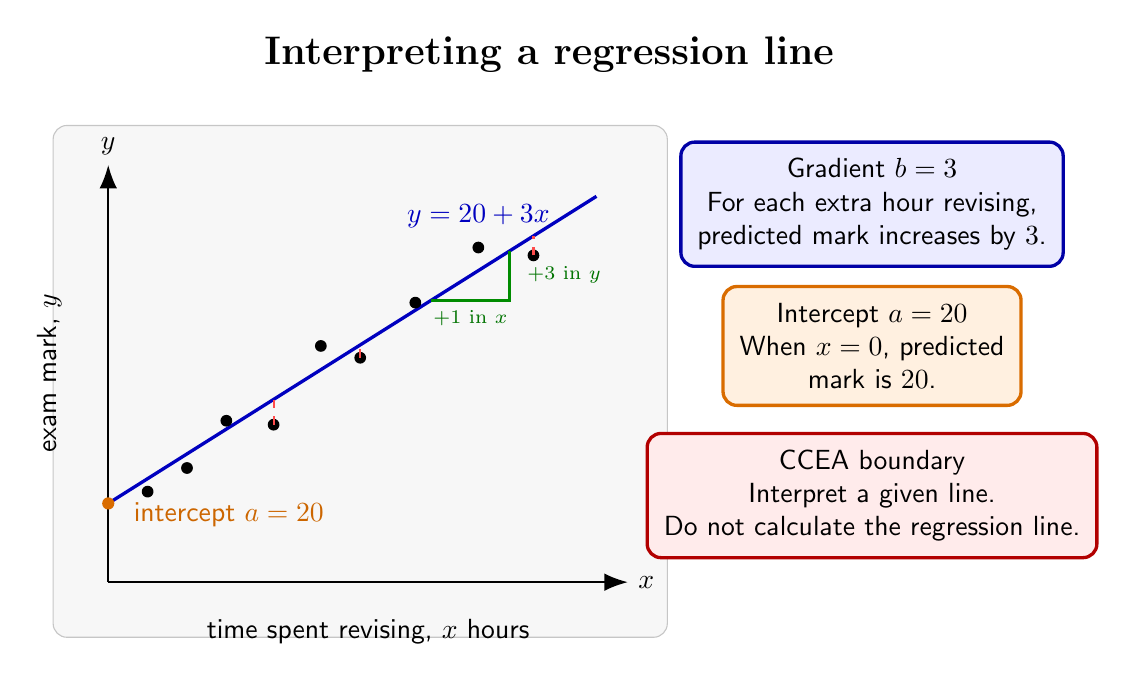
\begin{tikzpicture}[font=\sffamily,>={Latex[length=3mm]},point/.style={circle, fill=black, inner sep=1.5pt},card/.style={draw, rounded corners=5pt, very thick, align=center, inner sep=6pt}]
\node[font=\bfseries\Large] at (5.6,6.7) {Interpreting a regression line};
\draw[rounded corners=5pt, fill=gray!6, draw=gray!45] (-0.7,-0.7) rectangle (7.1,5.8);
\draw[->, thick] (0,0) -- (6.6,0) node[right] {$x$};\draw[->, thick] (0,0) -- (0,5.3) node[above] {$y$};
\draw[very thick, blue!75!black] (0,1.0) -- (6.2,4.9);\node[blue!75!black, font=\bfseries] at (4.7,4.65) {$y=20+3x$};
\foreach \p in {(0.5,1.15),(1.0,1.45),(1.5,2.05),(2.1,2.0),(2.7,3.0),(3.2,2.85),(3.9,3.55),(4.7,4.25),(5.4,4.15)}\node[point] at \p {};
\draw[red!70, dashed, thick] (2.1,2.0) -- (2.1,2.32);\draw[red!70, dashed, thick] (3.2,2.85) -- (3.2,3.01);\draw[red!70, dashed, thick] (5.4,4.15) -- (5.4,4.39);
\fill[orange!85!black] (0,1.0) circle (2.2pt);\node[orange!80!black, anchor=west] at (0.2,0.85) {intercept $a=20$};
\draw[green!55!black, very thick] (4.1,3.58) -- (5.1,3.58) -- (5.1,4.21);\node[green!45!black, font=\scriptsize] at (4.6,3.35) {$+1$ in $x$};\node[green!45!black, font=\scriptsize, anchor=west] at (5.2,3.9) {$+3$ in $y$};
\node[below] at (3.3,-0.35) {time spent revising, $x$ hours};\node[rotate=90] at (-0.75,2.65) {exam mark, $y$};
\node[card, fill=blue!8, draw=blue!65!black] at (9.7,4.8) {Gradient $b=3$\\For each extra hour revising,\\predicted mark increases by $3$.};
\node[card, fill=orange!12, draw=orange!85!black] at (9.7,3.0) {Intercept $a=20$\\When $x=0$, predicted\\mark is $20$.};
\node[card, fill=red!8, draw=red!70!black] at (9.7,1.1) {CCEA boundary\\Interpret a given line.\\Do not calculate the regression line.};
\end{tikzpicture}\end{document}
